% File: formatting-instruction.tex
\documentclass[letterpaper]{article}
\usepackage{aaai}

\usepackage{times}
\usepackage{helvet}
\usepackage{courier}
\usepackage{graphicx}
\pdfinfo{
/Title (Temporal Planning and Inferencing for Personal Task Management with SPSE2)
/Subject (ICAPS 2011)
/Author (Andrew Dougherty)}
% The file aaai.sty is the style file for AAAI Press 
% proceedings, working notes, and technical reports.
%
\title{Temporal Planning and Inferencing for Personal Task Management with SPSE2}
\author{Andrew Dougherty\\
FRDCSA Project\\
1125 Village Center Pkwy Unit 1.  Aurora, IL 60506\\
andrewdo@frdcsa.org\\
}
\setcounter{secnumdepth}{0}

\begin{document} 
\maketitle
\begin{abstract}
\begin{quote}

SPSE2 is a free and open source software system for personal task
management that uses publicly available temporal planning systems and
tools.  It provides a GUI for users to edit planning domains
consisting of assertions about goals and their interrelations and
temporal, cost and other constraints.  It also integrates calendar and
transportation planning information.  A voice-controlled mobile
application on the Android platform for goal setting, interactive
execution monitoring and replanning is currently under development.
The rest of this paper concerns details and planned features,
application areas and future work; as well as various other AI-related
technologies being used to extend the usefulness of the core
functionality.  For example, computational semantics software will
extract models of the meaning of the goals and translate into elements
of the planning language, and deontic logics will help to determine
the consistency of the goals and plans with the user's preferred
ethics and value systems.  The work is being conducted as part of the
Cognitive Prostheses research focus of the FRDCSA project.

\end{quote}
\end{abstract}

\section{Introduction}

This paper documents progress within the Formalized Research Database;
Cluster, Study and Apply project (FRDCSA) on applying existing AI
planning and scheduling tools to the domain of personal task
management.  We are developing this tool with three primary
communities in mind:

\begin{itemize}
\item The disabled (Pervasive Developmental Disorders)
\item The impoverished
\item Everyone else
\end{itemize}

Executive function (a.k.a. executive skills) is one life-critical
ability that is often impaired in those with Pervasive Developmental
Disorders (PDDs) such as Asperger Syndrome, High-Functioning Autism or
Schizophrenia.  ``Because the environment can be unpredictable,
executive functions are vital to human ability to recognize the
significance of unexpected situations and to make alternative plans
quickly when unusual events arise and interfere with normal
routines.''  Annecdotal evidence suggests that the executive function
in those without PDDs may also have room for improvement, especially
when compared to the optimal.  Furthermore, automated negotiation and
coordination of temporal constraints and privacy preferences may
further enhance the planning, scheduling and execution efficacy of
groups of persons.  Such improvements in local planning efficacy and
resource utilization could have macroscopic effects and relax
otherwise exacerbated resource conflicts.  Additionally, the
application of user-defined ethical analytics through computational
deontology offers a method to constrain the space of possible actions
that are available to intelligent personal agents.  Therefore,
development of a freely redistributable personal task management
system that interfaces with existing sources of data such as
calendars, routing applications and mobile phones could be a potential
way to improve the quality of life ubiquitously.

In additional to serving the disabled community, there are also those
who are practically disabled by poverty.  The proliferation of
Android-based smart phones with Wifi access has provided a vector to
provide the impoverished with practical life-planning technology.

\subsection{Overview of the FRDCSA Project}

\noindent The first major goal of the FRDCSA project, 10 years and
running, is to provide for better security and quality of life for all
sentient beings.  A major assumption is that artificial intelligence,
engineered correctly, can satisfice this goal.  To avoid polemics, we
concern ourselves with implementing a restricted form of weak AI.  The
approach, motivated by algorithmic information theory and
information-theoretic computational complexity of metamathematics
\cite{chaitin1974}, has two prongs - develop an increasingly complete
theorem proving system and library (called Formalized Research
Database (FRD)), and develop an increasingly complete collection of
practical software (Cluster, Study and Apply (CSA)).  I speculate that
the two approaches are theoretically equivalent by the Curry-Howard
ismorphism which seems to say that the classes of programs and proofs
are coextensive.  So the FRD ideally is a practical implementation of
Hilbert's program, which can never be completed, but which can, by
engineering a sequence of logics each more complete than the previous,
decide in the limit all problems which are not absolutely undecideable
(if any of those should exist).  This idea is similar to or the same
as an idea of Turing of creating a system of logics each more complete
than the previous and corresponding to constructible ordinals
\cite{turing1939}.  The CSA consists of a set of programs for building
and packaging most or all known freely available software systems and
datasets.

Because of the primary goal of the project and limitations to personal
productivity, it is necessary to develop tools that provide tangible
benefits to all persons and specifically those working on FOSS
software.  Hence we are developing a personal task management system.
Such a system is reasonably difficult to engineer, as evidenced by the
fact that the FRDCSA has almost 10 such systems in various stages of
completion.  So it is difficult to provide an accurate name for the
collection of functionality.  There are several primary FRDCSA systems
involved: Universal Language (UniLang), Shared Priority System Editor
version 2 (SPSE2), Free Knowledge-Based System (FreeKBS), Verber and
Planning, Scheduling and Execution (PSE).

\subsection{Overview of the SPSE2 System}

\noindent SPSE2 is a system for personal task management.  It provides
a GUI for users to edit planning domains.  The domains consist of
assertions in a knowledge base regarding goals and their constraints,
such as temporal and cost constraints.  The GUI allows users to
specify the constraints, and then the domain is converted into a PDDL
domain and a plan constructed.  Future versions will include a fully
functional interactive execution monitor that will walk the users
through the plans, and allow replanning, from headset voice controlled
cell phones.  The rest of this paper concerns various other AI-related
technologies being used to extend the usefulness of the core
functionality, application areas, and future work.

\begin{figure}[h!]
  \centering
      \includegraphics[width=84mm]{spse2.ps}
  \caption{Shared Priority System Editor v2}
\end{figure}

\section{System Architecture}

\subsection{UniLang}

\noindent The UniLang system is an interprocess communication system
for Perl ``agents''.  UniLang is loosely termed a multi-agent system,
patterned off of the Open Agent Architecture, but without most of the
Prolog-based communication capabilities (although it does have a
trivial FreeKBS-based knowledge interchange capability).  Most
subsystems communicate with each other through the {\bf Send} or {\bf
  QueryAgent} functions.

\subsection{Shared Priority System Editor}

One of the systems that has been under heavy development recently is
SPSE2.  The name derives from Justin Coslor's concept of Priority
Systems \cite{coslor2008}.  Our goal system is straightfoward, we have
a set of nodes which are goals, and a set of edges which are unary and
binary predicates on the goals.  We are extending SPSE2 to become a
knowledge editor, by adding several additional node types and
predicate sets and background knowledge.  Desired domains include:\\

\noindent {\it Alethic, Argumentation, Contexts, Critic, Deontic, Doxastic, Genealogy, IntelligentAgent, IntelligentTutoring, Inventory, Metamathematics, NetworkMapper, PICForm, Planning, POSI, SocialNetworking, SuppositionalReasoner, Tactics, Temporal, Workflow}\\

\noindent Here is related metadata from a sample goal in a planning
domain.  Suppose {\tt <REL>} is {\tt ("entry-fn" "pse" "38")}:

\begin{footnotesize}
\begin{verbatim}
("asserter" <REL> "unknown")
("goal" <REL>)
("has-NL" <REL> "ICAPS 2011 Paper")
("has-source" <REL>
 ("entry-fn" "sayer-index" "806"))
("depends" <REL> ("entry-fn" "pse" "17"))
...
\end{verbatim}
\end{footnotesize}

\subsection{FreeKBS}

Goals are straightforwardly expressed in natural language, and may be
marked with the unary predicate {\bf complete}.  The knowledge is
stored in FreeKBS.  FreeKBS can convert between several notations and
will eventually have more backends besides the current Vampire-KIF
backend, enabling reasoning over higher order and modal logics.
Vampire provides first-order theorem proving with equality.  The user
uses SPSE2 to develop a planning domain, which is stored in a FreeKBS
context (equivalent more or less to CYC's microtheories).

From this domain, we then generate a PDDL domain.  We are holding off
on implementing more complex models of the semantics of processes
until the basic system is completed.  Ideally we would like to be able
to model goals that are ongoing or come up repeatedly (i.e. do the
laundry).  For now, we simply take a given goal and record whether it
is completed or not.  There are other predicates involved, such as
putting goals in abeyance etc.  In order to generate a plan, SPSE2
translates its domain into one usable by Verber.

\subsection{Verber}

Verber, named after the late Senior Chess Master Richard Verber, is
basically a wrapper around various PDDL planners.  Verber provides a
set of Perl modules for building and interacting with PDDL domains
(and hopefully other planning formalisms eventually), for calling
various planners, and parsing the results.  It also houses a primitive
knowledge engineering aspect for constructing .verb format planning
domain libraries tailored to the specific domains required in the
project, such as movement discipline, goal tracking and meal planning.
the Verb format is a very lightly extended PDDL, which allows
importing other domains and problems and also a way to convert between
the scalar time values used by temporal planners and actual dates and
times.

Ideally Verber is capable of looking at goals and learning the average
and worst case durations of certain types of actions or events, and
incorporating this into the plan development.

Currently, there are several planners that are partially integrated,
but the one we have made the most use of LPG-TD so far
\cite{gerevini2004}.

\subsection{PSE}

\noindent PSE stands for Planning, Scheduling and Execution.  It is
one of the oldest of the FRDCSA systems and planning systems.  While
the original design using object-oriented Perl code has largely been
replaced with the PDDL-based approach through Verber, there still
remains a significant set of Emacs code within the namespace which
works with the new Verber model.  Before SPSE2 was written, this was
the primary way of interacting with the system.  Several interfaces
were developed for manipulation of goals.  All of these codes are
based on Emacs.  Significant to note are the functions for rapidly
asserting relations between goals.  In order for readability, a
function exists which, when the Emacs point is moved over the natural
language description of a goal, will be the entry ID of the goal onto
a kind of stack.  Additional commands operate on the contents of the
FreeKBS stack.

\section{System Interfaces}

\subsection{Calendar Synchronization}

In order to improve the utility of Verber, I have developed a calendar
synchronization feature.  This allows us to synchronize with ICS
Calendars or Google Calendars, the ICS files of which are obtained and
then translated into the SPSE2 domain representation.  In order to
schedule an event occuring at a certain time, it is translated from
the datetime information into the offset and scale of the scalar
planning time value.  The event start date is marked using PDDL timed
initial literals.

\begin{footnotesize}
\begin{verbatim}
(at 1.00 (possible <EVENT>))
(at 2.00 (not (possible <EVENT>)))
\end{verbatim}
\end{footnotesize}

Additionally the planning domain includes the following precondition
for the durative action {\bf Complete}.

\begin{footnotesize}
\begin{verbatim}
(over all
 (or
  (not (has-time-constraints ?e1))
  (possible ?e1)))
\end{verbatim}
\end{footnotesize}

Here is an example of the time constraints that are asserted by the
DateTime interface.

\begin{footnotesize}
\begin{verbatim}
("end-date"
 ("entry-fn" "pse" "38")
 "TZID=America/Chicago:20101129T120000")
\end{verbatim}
\end{footnotesize}

\subsection{Notification Manager}

\noindent We have partially completed a Perl/TK-based notification
manager patterned off of the Android notification manager.  Ideally,
it should be able to synchronize with the Android notification
manager.

Certain tasks that regularly occur are regularly added to the SPSE2
planning context by a cron job.  The custom Cron like format includes
information on how much warning time should predate the beginning of
the possibility of completing a task.  Ideally, we would monitor.

\begin{figure}[h!]
  \centering
  \includegraphics[width=84mm]{notification-manager.ps}
  \caption{Notification Manager}
\end{figure}

\subsection{Deontic and Teleologic Logics}

\noindent We would like to place certain ethical constraints on
possible actions, in order to provide agents with a support system.
To do this, we wish to formalize various systems of morality in terms
of deontic logics, and to provide an evaluation function which
evaluates individual actions and plans against various moral systems.
Therefore, the user simply declares which moral systems to which they
agree, and the system then evaluates the actions.  To illustrate a
very simple example, we might consider the Ten Commandments,
especially the rule: ``Thou shalt not kill''.  This would be manually
translated to ``Someone or something murdered''.  This is converted to
a logic form LF and then we assert:

\begin{footnotesize}
\begin{verbatim}
(implies <LF> (rule-activated <RULE-NUMBER>))
\end{verbatim}
\end{footnotesize}

We then determine whether this rule is activated use semantic textual
entailment recognition.  In our case, we would then load the logic of
the plan and all enumerable consequences, convert to logic form,
instantiate the variables with their valuations, add contingent
background knowledge, and query: (rule-activated ?X).  Of course, in
practice this will be much more complicated.

Besides considering general obligations and prohibitions (deontics),
it will also be useful to consider a means-ends analysis (teleologics
I believe).

\subsection{World State Comparision and Value Systems}

\noindent An intended capability is to reason more intelligently about
the value of a given plan or outcome.  In trying to evaluate various
actions to determine which is morally superior, it begs the question
of which world-states and histories are preferable.  To evaluate this,
we need to develop a general comparison function.  To reduce the
evaluation to a total order would be somewhat dualistic - but
ultimately we would like the user to be able to choose among possible
worlds - or rather provide rules which in some sense order them.  A
very important task is to reason with the consequences

\subsection{House Rules}

\noindent An intended system consists of standard house rules and
other constraints on the creation and execution of plans.  The house
rules system seeks to take standard rules related to planning.  For
instance, a house rule of remember to leave the lid of the washing
machine open after removing

\subsection{Android Bluetooth Headset Based Interactive Execution Monitor}

\noindent In order to provide a usable interface to the plans, I am
developing an application for the Google Android mobile operating
system, for recording new goals, walking the user through generated
plans, and initiating replanning.  Currently, the system uses XMLRPC
to agentify the phone and communicate with UniLang.  The user intiates
voice recognition by pressing a certain combination of buttons on
their bluetooth headset.  Recognition results are then sent via XMLRPC
to a special UniLang client which forwards it to the main UniLang
system and on to its intended agent, in this case, a special agent for
interpreting voice commands.  Initiating communication to the phone is
accomplished either through registering the phone with a Dynamic-DNS
provider, or by polling from the phone to the server.  Voice commands
for controlling the process of planning, replanning and the
interactive execution monitor will be developed.

\subsection{Location Logic}

\noindent Location Logic is a system for inferencing with the
semantics of the users location as reported by the GPS, as contrasted
to their waypoints, and so on.  It asserts theorems observed regarding
the GPS realtime tracks (through Google Latitude), such as whether
certain waypoints are being approached, visited, departed, etc.  It
interfaces naturally with the todo system.

Here is an example use case.  Suppose both Alice and Bob are using
mobile phones (most likely Android devices) with the LocationLogic
system installed.  Furthermore, they have a hands-free voice
controlled task list, similar to or the same as the Voice Control task
system that is under development.  Both Alice and Bob are wearing
bluetooth headsets.

So suppose Alice is out of milk, but she doesn't know this right away.
(Perhaps her roommate drank the last of it, and did not or could not
tell her yet).  Meanwhile, Bob is out running errands of his own.

Alice wakes up and comes down the stairs and goes to get some cereal.
She pours the bowl of cereal and then looks in her refrigerator.  She
realizes that the milk is empty and has not been thrown out.

Disappointed, she taps a button on her bluetooth headset.  She quickly
hears it say ``Yes?''.  Alice says: ``pantry remove item milk'', to
which her headset says, ``Confirm remove milk from pantry
inventory?''.  Alice says ``yes''.  ``Milk removed'' says the headset.

When Alice told the system that she was out of milk - the system
realized according to various considerations that she should buy some
more milk.  It therefore automatically added the goal ``get milk'' to
the system.

\begin{figure}[h!]
  \centering
  \includegraphics[width=84mm]{location-logic.ps}
  \caption{Location Logic Prototype}
\end{figure}

Now because Alice and Bob are friends, they have already told their
Shared Planning Systems that they can collaborate on many matters, one
of which is food inventory.  So, Alice's planning agent sent a
broadcast to all of her friends that she shares this kind of
information with.  It was stated simply as the goal that there is a
fresh jug of milk in Alice's refrigerator.  The various agents
therefore add this goal to their own planning systems.  (Note I
haven't worked out the details of this, but it should follow naturally
as I complete simpler sub-problems).  They all develop a new plan
which incorporates Alice's request.  Then they compare plans.  Bob's
planning agent realized that because Bob was nearby a grocery store,
and that he didn't have other things that couldn't be slightly
postponed, that he could pick it up and drop it off to Alice's house.
So all the planning agent's agree that this is the best plan...

Bob and Alice both get a message suggesting that this action be taken.
Once both have agreed, it is added to the planning system, even
including so much as to tell Bob's cell phone agent which type of milk
Alice would like.

Bob then purchases the milk and then swings by Alice's place on his
way to work.  For now, we can assume Alice pays him cash - but in the
future we will use an automated loan/payment system currently under
development.

Here follows an example Location Logic rule.

\begin{footnotesize}
\begin{verbatim}
(implies
 (and
  (leaving ?AGENT ?LOCATION)
  (isa ?LOCATION movie-theatre)
  (has-performed-action ?AGENT
   "silence cell phone at movie theatres")
  ;; (> (sitting-still) (minute 1))
  )
 (perform-action "add-to-pending-tasks"
  "unsilence cell phone \
   when leaving movie theatres"))
\end{verbatim}
\end{footnotesize}

\subsection{Federated Transportation Planning}

\noindent To make the system more useful, especially to the homeless,
I am working on integrating a federated transporation planning option.
This should naturally understand way points, and be able to generate
queries to a public or private transportation routing system in order
to populate the model with the timing constraints.  Ideally actual bus
positions and timing projects etc could be integrated - and replanning
initiated as needed.  Previously, the FRDCSA BusRoute bus timetable
planner was integrated with Verber, but now we are interested in
interfacing with Google's public transportation planner.

\subsection{Automatic Execution of Tasks}

\noindent One interesting area of the system is to take the planning
capabilities of the system, and existing plan instantiation libraries,
and use this information to achieve automatic completions of portions
of the plan, and also a generic user 

\section{Related Technologies}

\subsection{Semantic Web Ontologies}

\subsection{Textual Entailment Recognition}

\subsection{Computational Semantics Via Logic Forms}

\section{Systems Using SPSE/Verber/PSE}

\subsection{POSI Collaboration}

\noindent A project that is using the tools of the FRDCSA is POSI.
POSI stands for POSI Open Source Initiative.  It is a system for
representing the goals, interests and abilities of its users, as
distilled from their writings and provided information.  The idea is
to establish the necessary and sufficient information to form dynamic
multiagent teams to solve problems that are shared between multiple
persons.  SPSE is the Shared Priority System Editor.  Priority Systems
are essentially networks of goals and constraints on these goals.
Future versions of SPSE will be able to simultaneously edit the same
Shared Priority Systems.  An essential feature of the system is
identifying when different users have specified the same or related
goals.  This is accomplished chiefly using the nascent technology of
Textual Entailment Recognition, as well as through breaking down
individual goals into more clearly defined or achievable steps.

As such, the Goals, Interests and Abilities (GIAs) of the users are
modelled using ontological tools.  SPSE2 itself will have the ability
to edit domains besides temporal planning, including different
ontologies, including those of the POSI.

I am most interested in collaborating with those in the AI planning
and scheduling field on open source tools, and would like to use POSI
to help achieve that.

\subsection{Akahige Medical System}

The planning system and interactive execution monitor have several
applications.  One intended application is the Akahige Medical System.
One capability of the Android phone-based general purpose help system
is to launch a medical help system in the event that any symptoms
occur and are complained about by the user.  The symptoms can be run
through a standard or custom medical diagnostic program (such as
Diagnosaurus or the planned Akahige Model-Based Diagnostic and Fault
Localization software).  The result of the diagnostic procedure may
require an emergency response, or a more abated response.  In either
case, instructions for the given emergency or situation will exist
within the system and the user will be guided by the interactive
execution monitor to complete these tasks, or referred to
documentation.

\subsection{Gourmet Meal Planner}

Another area of interest is meal planning.  The FRDCSA project has a
meal planner, called Gourmet.  Gourmet is intended to improve the diet
of users.  It will interface with our inventory management component
for pantry management.  We have a database of 150,000 or so recipes in
mealmaster format (the SOAR archive).  Work is progressing on
developing a foodstuffs ontology, on which to map the ingredients and
intermediate foodstuffs of the recipe.  Mapping to nutrient databases
such as the SR23 and also to product databases such as
UPCdatabase.com, in addition to formalizing the recipe steps into
discrete planning operations, will provide all the resources required
to achieve interactive recipe execution through the Android interface.
The formalization of recipe steps will hopefully be attempted by
training CMU's StackedFrameParser on the CURD/MILK dataset of
annotated recipes.  They use a medium grained language called CURD
which expresses a set of abstracted operations on food
\cite{tasse2008}.  This includes the intermediate foodstuffs.  Then
arbitrary English recipes may be attempted.  As some other open source
meal planners have well established user bases, this automatic
annotation could be performed and cached by a webserver (as the
StackedFrameParser seems to require 8GB RAM), and could be augmented
and trained by user corrections given a sufficient GUI and upload
mechanism.

http://frdcsa.org/frdcsa/internal/gourmet

\subsection{Paperless-Office System}

Another FRDCSA project that will make use of the planning technology
is the Paperless-Office.  With this system, which already functions to
scan, OCR, search and edit documents, it will be possible to specify
workflows - such as certain documents requiring to be filled out and
sent by certain times.

http://freshmeat.net/paperless-office

\begin{figure}[h!]
  \centering
      \includegraphics[width=84mm]{paperless-office.ps}
  \caption{Paperless-Office}
\end{figure}

\subsection{Story Understanding and Generation}

An area of interest is in story understanding and generation (not to
mention poetry).  So for instance, the exposition structure of this
LaTeX paper was modelled using a planning domain, although specialized
domains are/will be developed.  These domains necessarily use the
various other the domains, such as multiagent modeling capabilities,
of SPSE2 - to model what the authors intended effects are on the
audience and to generate stories that match these goals.

INCLUDE IMAGE HERE

\subsection{SystemX Intelligent Tutoring Systems}

Work has been ongoing on Arbitrary Document Understanding.  Being able
to represent the argument structure of a text, and also the facts and
relations of the text, enables the generation of temporal plans for
teaching subjects at various granularities based on various learning
objectives and timing constraints.  A prototype system called Study
has been developed.  SystemX will use the SPSE2 or its derivatives.

\section{Conclusions and Future Work}

\noindent We are close to completing usable Perl/TK, Emacs and Android
systems for editing goals, adding temporal constraints, generating
plans, and walking the user through them.  The chief obstacle to the
release of this work, other than the work itself, is that the software
developed depends on a large set of heavily interconnected yet
unreleased software dependencies.  I would like to see a proper
requirements engineer process initiated (as the project management for
SPSE2 is currently performed within SPSE2 itself - a chicken and egg
problem).  I need to get a working phone and complete the interactive
execution monitor - as well as resolve some pernicious bugs.

\subsection{Automatic PDDL Domain Construction Via Computational Semantics}

\noindent Although goals are simply evaluated in a boolean context, we
are working on providing a more detailed interpretation of the
semantics of the goals.  Ideally, we would convert the natural
language contents of goals and other node types into a logical
semantic representation, such as logic forms (LFs), and from the LFs
construct the PDDL domains and problems.

\subsection{Suppositional Reasoner}

\noindent The suppositional reasoner seeks to incorporate more
positional evaluation and analysis of domain invariants, domain
specific knowledge and so on, into the planning process.  It ideally
would function as a plan development and critiquing interface for
real-life problems, hopefully allowing the evaluation of any decision
making process.  It is being calibrated on domains like Chess and Go
that have a substantial literature that may be formalized and in which
feedback on efficacy is relatively short.  From a search point of
view, it is not very interesting, for starters we are going to
implement some standard searches.  But attempting to hybridize the
search with positional information is interesting.  We are taking
annotated chess games and formalizing the annotations to develop
knowledge that may be tested and applied to the situation.

We also have a formalization for theorem proving over these models.
It is the same formalization that being used to perform natural
language understanding within the project.  It is the Sayer system.

\subsection{Temporal Conformant Planning}

One desired capability is temporal conformant planning, and tools for
exploring the set of actions possible to the agent at each state, and
reasoning with the consequences of various choices at that point.
This naturally reflects back to the suppositional reasoner and the
valuation system.

%% Basic functionality in leiu of temporal conformant planners is to fork
%% domain at each environmental decision point and generate plan - store
%% plan hierarchy, also which nodes have no plan and require domain
%% reengineering

\section{Acknowledgments}

\noindent I am grateful especially to Aloysius Flori, Rachel Beil, and
my immediate family who have variously sustained me during periods of
homelessness and insolvency.  I am grateful to Justin Coslor who has
provided the inspiration for countless systems and programs and has
developed a formal theory of context.  I am grateful to the CMU
community for its grace and tolerance during my periods of
homelessness.  I am grateful to Jim Oberweis and the late Richard
Verber for their support and mentorship with chess.  I am grateful to
the many persons who showed me kindnesses when they were under no
obligation to do so.

I wish firstly to thank all of the researchers who have made progress
in this field and also those who have released software under freely
redistributable licenses.  Such licenses make the work of an open
source developer much easier - we may simply include your software
into our own.

I am indebted to the authors of LPG for making their temporal planning
system available.

\bibliographystyle{aaai}
\begin{thebibliography}{}

\bibitem[\protect\citeauthoryear{Chaitin}{1974}]{chaitin1974}
Chaitin, G.
\newblock 1974.
\newblock Information-theoretic limitations of formal systems.
\newblock {\em Journal of the ACM} 21:403--424.

\bibitem[\protect\citeauthoryear{Coslor}{2008}]{coslor2008}
Coslor, J.~M.
\newblock 2008.
\newblock {\em Possibility Thinking}.
\newblock Lulu.com.

\bibitem[\protect\citeauthoryear{Gerevini, Saetti, and
  Serina}{2004}]{gerevini2004}
Gerevini, A.; Saetti, A.; and Serina, I.
\newblock 2004.
\newblock {LPG-TD}: a fully automated planner for {PDDL}2.2 domains.
\newblock {\em 14th Int. Conference on Automated Planning and Scheduling
  (ICAPS-04)}.

\bibitem[\protect\citeauthoryear{Tasse and Smith}{2008}]{tasse2008}
Tasse, D., and Smith, N.~A.
\newblock 2008.
\newblock {SOUR CREAM}: Toward semantic processing of recipes.
\newblock Technical Report~5, Carnegie Mellon University, Pittsburgh, PA.

\bibitem[\protect\citeauthoryear{Turing}{1939}]{turing1939}
Turing, A.
\newblock 1939.
\newblock Systems of logic based on ordinals.
\newblock In {\em Proc. London Math. Soc.},  161--228.

\end{thebibliography}

%% \noindent Chaitin, G. J. 1974. Information-Theoretic Limitations of Formal Systems. {\it Journal of the ACM} Vol. 21, 403-424.\\

%% \noindent Coslor, J. M. 2008. Possibility Thinking. {\tt http://picform.org}.\\

%% \noindent Alfonso Gerevini, Alessandro Saetti, Ivan Serina. 2004. LPG-TD: a Fully Automated Planner for PDDL2.2 Domains {\it 14th Int. Conference on Automated Planning and Scheduling (ICAPS-04)}\\

%% \noindent Sally McGhee, John Wittry. 2007.  Take Back Your Life: Using Microsoft Office Outlook 2007 to get organized and stay organized.\\

%% \noindent Noah Slater. 2007.  CURD:\\

%% \noindent Turing, A. 1939. Systems of Logic Based On Ordinals. {\it Proc. London Math. Soc. (1939) s2-45 (1):} 161-228.\\

\end{document}
